\subsection{Fits\-Slice  Class Reference}
\label{class_fitsslice}\index{FitsSlice@{Fits\-Slice}}
Memory saving traversal of a fits image. 


{\tt \#include $<$fitsslice.h$>$}

Inheritance diagram for Fits\-Slice::\begin{figure}[H]
\begin{center}
\leavevmode
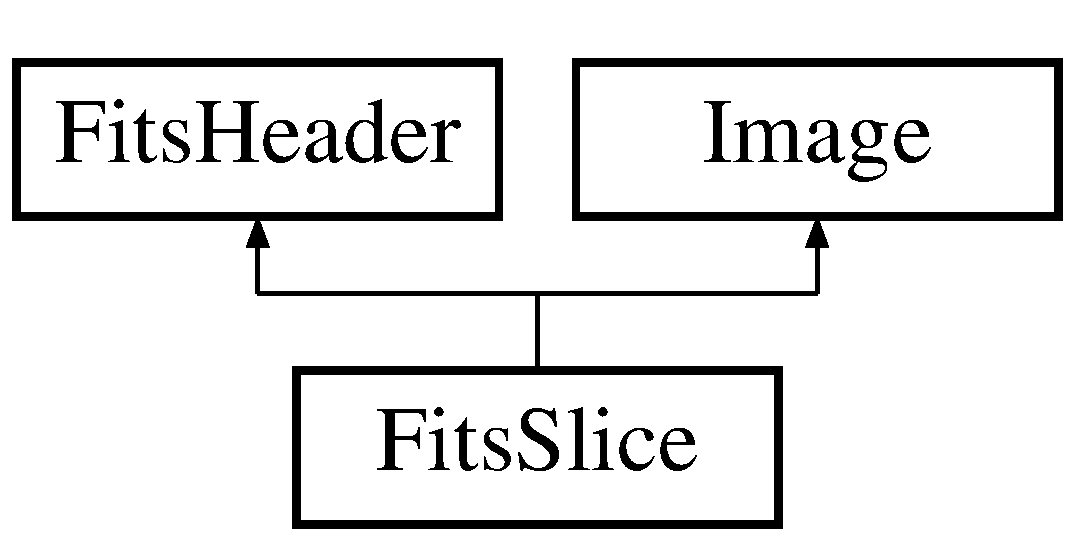
\includegraphics[height=2cm]{class_fitsslice}
\end{center}
\end{figure}
\subsubsection*{Public Methods}
\begin{CompactItemize}
\item 
\index{FitsSlice@{FitsSlice}!FitsSlice@{Fits\-Slice}}\index{FitsSlice@{FitsSlice}!FitsSlice@{Fits\-Slice}}
{\bf Fits\-Slice} (const string File\-Name, const int Slice\-YSize, const int Overlap)\label{class_fitsslice_a0}

\begin{CompactList}\small\item\em constructor. Overlap is the number of rows in common to successive slices (usually 0).\item\end{CompactList}\item 
\index{LoadNextSlice@{LoadNextSlice}!FitsSlice@{Fits\-Slice}}\index{FitsSlice@{FitsSlice}!LoadNextSlice@{Load\-Next\-Slice}}
int {\bf Load\-Next\-Slice} ()\label{class_fitsslice_a1}

\begin{CompactList}\small\item\em load next slice into memory.\item\end{CompactList}\item 
\index{SliceSize@{SliceSize}!FitsSlice@{Fits\-Slice}}\index{FitsSlice@{FitsSlice}!SliceSize@{Slice\-Size}}
int {\bf Slice\-Size} () const\label{class_fitsslice_a2}

\begin{CompactList}\small\item\em the current slice size (differs from the constructor value at last slice).\item\end{CompactList}\item 
\index{ImageJ@{ImageJ}!FitsSlice@{Fits\-Slice}}\index{FitsSlice@{FitsSlice}!ImageJ@{Image\-J}}
int {\bf Image\-J} (const int j) const\label{class_fitsslice_a3}

\begin{CompactList}\small\item\em the coordinate in the full image of row j in present slice.\item\end{CompactList}\item 
\index{LastSlice@{LastSlice}!FitsSlice@{Fits\-Slice}}\index{FitsSlice@{FitsSlice}!LastSlice@{Last\-Slice}}
bool {\bf Last\-Slice} () const\label{class_fitsslice_a4}

\begin{CompactList}\small\item\em are we in the last slice?\item\end{CompactList}\end{CompactItemize}


\subsubsection{Detailed Description}
Memory saving traversal of a fits image.

This class is intended to access an image in a fits file, but only a slice of the image will reside in memory at a time. To be used when many images have to be accessed at the same time, in parallel (see {\bf Fits\-Parallel\-Slices} {\rm (p.\,\pageref{class_fitsparallelslices})}), or maybe to traverse a very big image. 



The documentation for this class was generated from the following file:\begin{CompactItemize}
\item 
{\bf fitsslice.h}\end{CompactItemize}
